\section{Supplementary Information}
\begin{suppfigure}
    labelled and    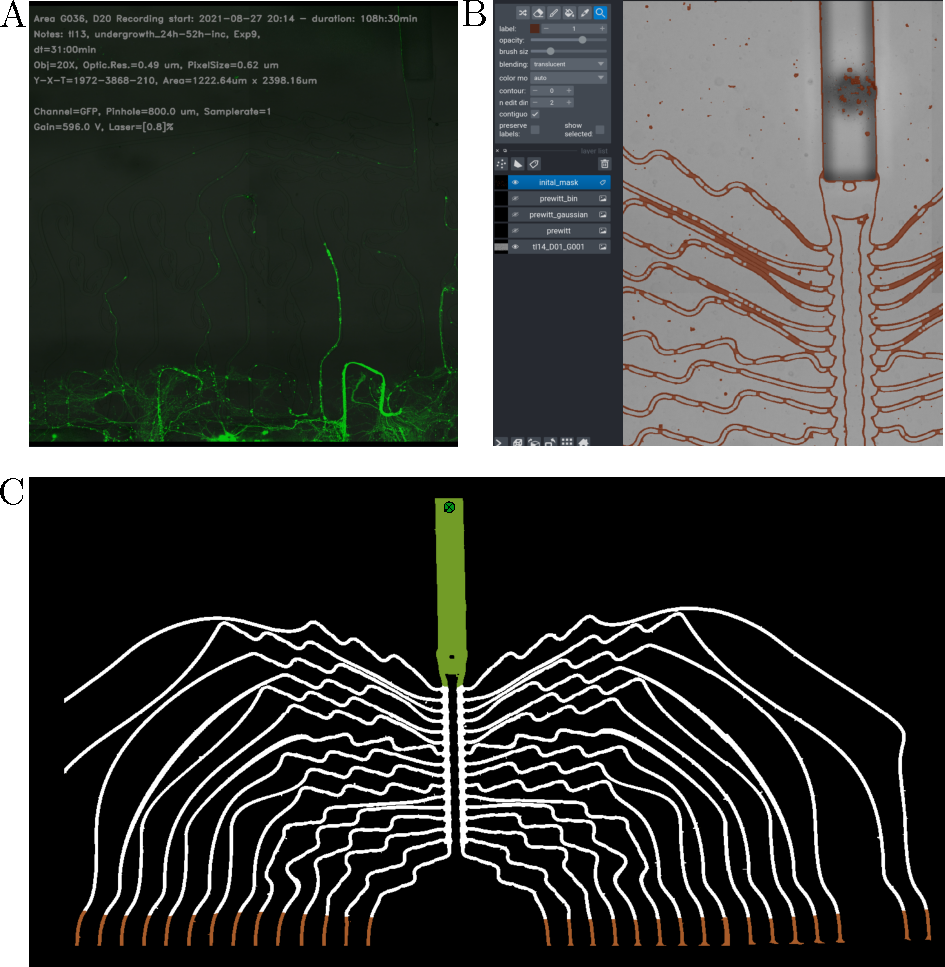
\includegraphics{SF_intial_tl_preprocessing.pdf}
    \caption[Initial timelapse preprocessing steps]{Initial timelapse
             preprocessing steps. \textbf{A} A snapshot of the exported video
             including the relevant metadata of the recording. \textbf{B} The
             napari image viewer interface with the edge segmentation layer in
             brown. \textbf{C} The manually segmented binary mask of the micro
             channels in non-black, the output channel in green, and the exiting
             channels in brown. The green dot in the output channel marks the
             target point of the PDMS design.}
    \label{SF_intial_tl_preprocessing}
\end{suppfigure}

\begin{suppfigure}
    \includegraphics{SF_labelling.pdf}
    \caption[Axon growth cone labelling]{Axon growth cone labelling. \textbf{A} shows a
             snapshot of the napari image viewer during labelling. Each circle
             represents a growth cone label, the color corresponds to the
             identity. Each axon identity is saved as a napari-Points layer
             which are listed on the left. \textbf{B} illustrates the axon
             identify lifetime. A green point on this pixel map indicates that a
             label exists for the matching axon identity and frame. The
             three clusters originate from the concatenation of three
             PDMS microstructure timelapse videos. }
    \label{SF_labelling}
\end{suppfigure}

\begin{suppfigure}
    \includegraphics{SF_training_data.pdf}
    \caption[Labelled training data examples]{Labelled training data examples.
             \textbf{A} shows the first frame of the training data sequence.
             Each box represents a growth cone, the color indicates the identity
             over consecutive frames. \textbf{B} shows the last frame of
             Dataset1. \textbf{C} shows the last frame of Dataset2, PDMS micro
             structure 1 (compare Table \ref{datasets_table}). \textbf{D} shows
             the last frame of Dataset2, PDMS micro structure 2. Gridsize = 317
             $\rm\upmu m$.} 
    \label{SF_training_data}
\end{suppfigure}

\begin{suppfigure}
    \includegraphics{SP_ax_reconstructions.pdf}
    \caption[Axon reconstruction from growth cone track]
    {Axon reconstruction from growth cone track. \textbf{A} For clarity, only a
    subset of identified axons is drawn.} 
    \label{SP_ax_reconstructions}
\end{suppfigure}



\begin{suppfigure}
    \includegraphics{SF_growthspeed.pdf}
    \caption[Axonal growth velocity]
    {Axonal growth velocity. Significance is not shown.} 
    \label{SF_growthspeed}
\end{suppfigure}


\begin{suppfigure}
    \includegraphics{SF_naxons.pdf}
    \caption[Axon outgrowth frequency]
    {Axon outgrowth frequency. Significance is not shown.} 
    \label{SF_naxons}
\end{suppfigure}


\begin{suppfigure}
    \includegraphics{SF_stagnation.pdf}
    \caption[Number of axons stagnating]
    {Number of axons stagnating. Significance is not shown. Top right plot shows
    counts of axons growing incorrectly (red), and correctly (green) for a
    feature that did not show significant effects.} 
    \label{SF_stagnation}
\end{suppfigure}

